\documentclass[11pt]{article}
\usepackage[utf8]{inputenc}
\usepackage[ngerman]{babel}

\usepackage{amsmath,amsthm,amssymb,amsfonts}

\usepackage{graphicx}
\graphicspath{{abb/}}
\usepackage{float}
\usepackage{tikz}

\usepackage{fancyhdr} % For headers and footers
\usepackage{geometry}
\usepackage{listings}
\usepackage{hyperref}
\hypersetup{
    linkcolor=blue,     
    urlcolor=cyan,
}

\geometry{
    a4paper, % Change this if you intend to print on a different paper size, such as letter paper.
    left=20mm,
    right=20mm,
    top=30mm,
    bottom=30mm,
}

\title{Dynamik - Impuls}
\author{Emil Staikov}
\date{10. Mai 2021}

\begin{document}
\maketitle

\section{Definition}
Der Impuls $\vec{p}$ eines Objekts ist definiert als das Produkt aus Masse und Geschwindigkeit dieses Objekts, also 
\begin{equation*}
    \vec{p} = m\vec{v} 
\end{equation*}
bzw. für eine Dimension (hier $x$) 
\begin{equation*}
    p_x = mv_x
\end{equation*}
Für ein System aus $n$ Objekten ist der Gesamtimpuls $\vec{p}_s$ die Summe der Impulse der einzelnen Objekte, also 
\begin{equation*}
    \vec{p}_s = p_1 + p_2 + ... + p_n = m_1\vec{v}_1 + m_1\vec{v}_1 + ... + m_n\vec{v}_n
\end{equation*}

\section{Impulserhaltung}
Bekanntlich ist die Beschleunigung die Änderung der Geschwindigkeit, also
\begin{equation*}
    \vec{a} = \frac{\Delta \vec{v}}{\Delta t}
\end{equation*}
Betrachten wir nun die Änderung des Impulses im Fall konstanter Masse: 
\begin{equation*}
    \frac{\Delta \vec{p}}{\Delta t} = \frac{\Delta m\vec{v}}{\Delta t} = m \frac{\Delta \vec{v}}{\Delta t} = m\vec{a}
\end{equation*}
Das ist aber nach Newtons zweitem Axiom genau die Kraft! Die Kraft ist also die Änderung des Impulses. Wenn wir nun einige Objekte, also ein System von Objekten betrachten, finden wir zwei Arten von Kräften: Kräfte zwischen Objekten des Systems (innere Kräfte), sowie Kräfte von außen (äußere Kräfte). Wenn unser System ein Inertialsystem ist, was für unsere Zwecke praktisch immer der Fall ist, exisitert nach Newtons drittem Axiom stets eine entgegengesetzt gleiche innere Gegenkraft. Die Summe aller inneren Kräfte ist also null. Wenn also die Summe der äußeren Kräfte auf das System ebenfalls null ist, so ist die Summe aller Kräfte in dem System null, wodurch auch die Änderung des Impulses null ist. Kurz zusammengefasst: \\\\ 
\textbf{Impulserhaltungssatz:} In einem Inertialsystem gilt: 
\begin{equation*}
    \sum_{\text{äußere Kräfte}} F = 0 \implies \frac{\Delta \vec{p}}{\Delta t} = 0 \text{, also } \vec{p} = \text{const.}
\end{equation*}

\section{Ein Beispiel}
Ein $5g$ schweres Geschoss wird mit Geschwindigkeit $100\frac{m}{s}$ in einen $1kg$ schweren Block geschossen. Wie schnell bewegt sich dieser Block direkt nachdem das Geschoss ihn trifft? 
\begin{figure}[H]
    \centering
        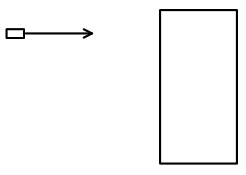
\includegraphics[width=0.3\textwidth]{impuls-geschoss.png}
\end{figure} 
Jegliche Bewegungen und folglich auch Impulse sind eindimensional, wir können also direkt mit den Größen rechnen ohne sie als Vektoren zu behandeln. Der Impuls $p$ des Systems vor dem Auftreffen ist die Summe der Impulse von Geschoss und Block: 
\begin{equation*}
    p = p_{Geschoss} + p_{Block} = 0.005kg \cdot 100 \frac{m}{s} + 0 = 0.5 \frac{kg\cdot m}{s}
\end{equation*}
Auf das Geschoss wirkt die Gravitationskraft, eine Auftriebskraft durch die Luft, sowie die Kraft durch den Block beim Auftreffen. Die Änderung des Impulses durch Gravitationkraft und Auftriebskraft ist vernachlässigbar klein. Die Kraft durch den Block auf das Geschoss ist entgegengesetzt gleich zur Kraft durch das Geschoss auf den Block, in Summe heben diese sich also auf. Auf den Block wirkt auch eine Gravitationskraft, der Block steht aber z. B. auf einem Tisch, welcher wieder eine Gegenkraft ausübt. Der Tisch hat ebenfalls ein Impuls von null, daher ändert das Einschließen des Tisches in unser System nicht den Gesamtimpuls. Insgesamt folgern wir, dass wir Impulserhaltung anwenden können. In Aufgaben müsst ihr das meistens nicht so extensiv begründen, ihr solltet es aber im Hinterkopf behalten. \\\\
Nach dem Auftreffen bleibt das Geschoss im Block stecken, die Gesamtmasse des Objekts ist dann $1.005kg$. Dieses System hat wie soeben begründet den Impuls $p = 0.5 \frac{kg\cdot m}{s}$. Jetzt können wir die Geschwindigkeit $v$ des resultierenden Objekts berechnen: 
\begin{equation*}
    0.5 \frac{kg\cdot m}{s} = 1.005kg \cdot v \\
    \iff v = \frac{0.5}{1.005} \frac{m}{s} \approx 0.498 \frac{m}{s}
\end{equation*}
\end{document}